\begin{figure}[t]
	\centering
	\addtolength{\tabcolsep}{-3pt}
	\begin{tabular}{c}
		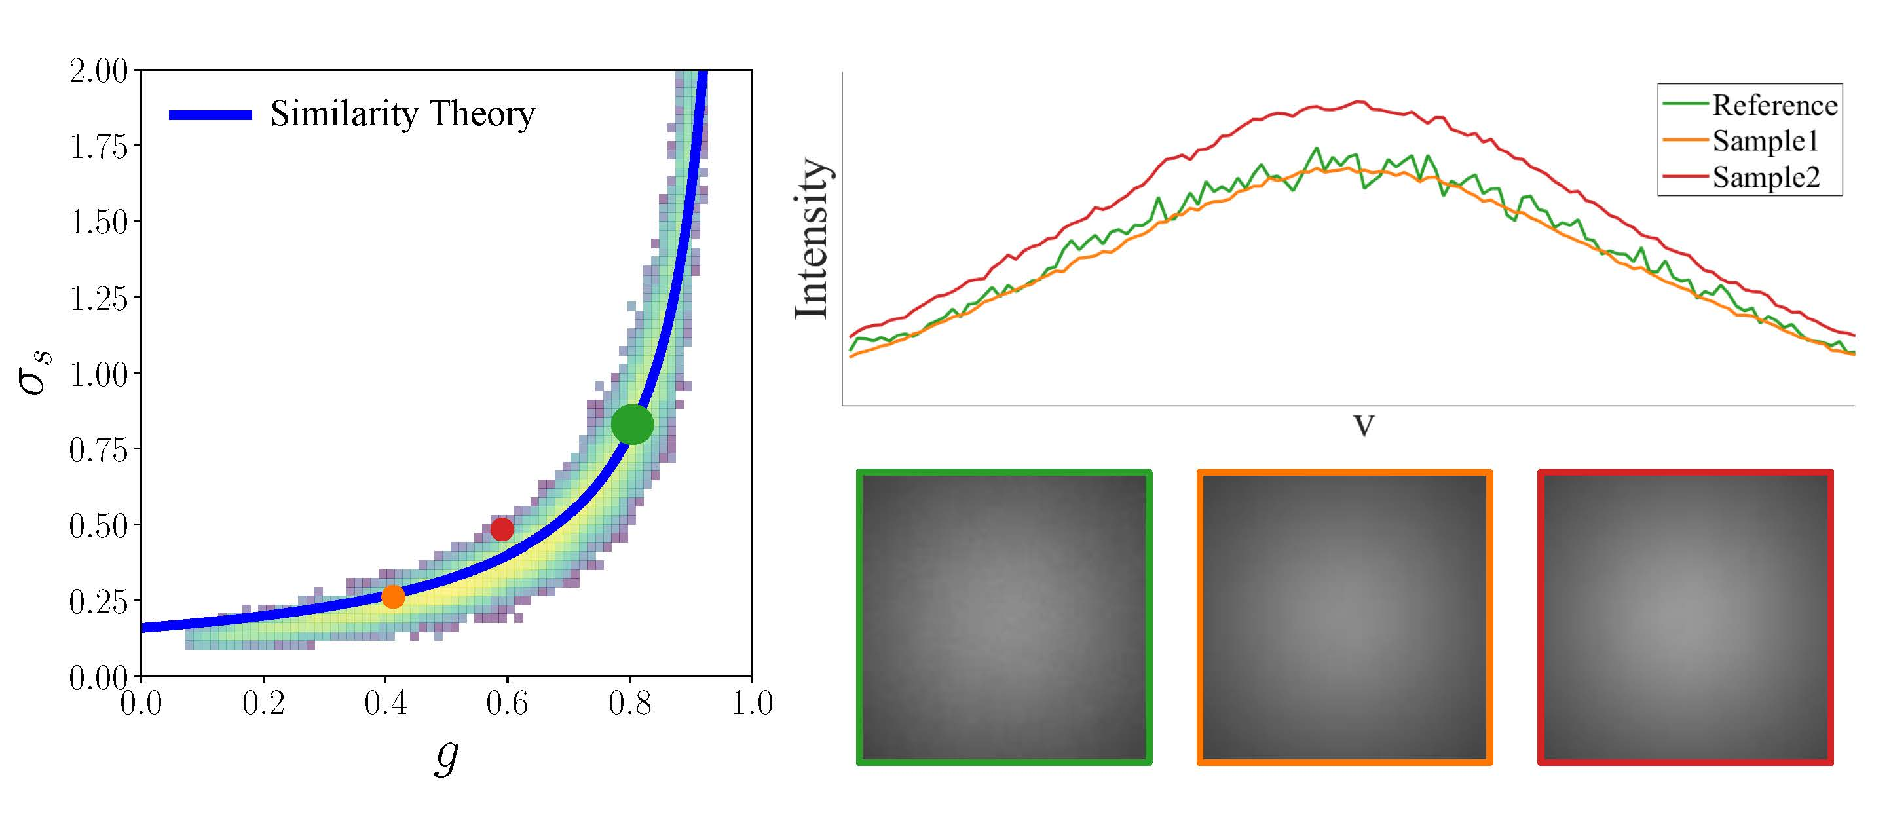
\includegraphics[width=0.98\columnwidth]{scatter/scatter.pdf}
	\end{tabular}
	\captionsetup{labelfont=bf,textfont=it}
	\caption{\label{fig:scatter}
		A motivating example of a scattering material with two estimated parameters (scattering coefficient and phase function parameter). The posterior distribution sampled with our method for three synthetic input images is able to detect the full structure of the parameter space, matching the predictions from similarity theory.
	}
\end{figure}

%\begin{figure}[t]
%	\centering
%	\addtolength{\tabcolsep}{-3pt}
%	\begin{tabular}{c}
%		\includegraphics[width=0.9\columnwidth]{images/scatter/image.png}
%	\end{tabular}
%	\caption{\label{fig:scatter2}
%	}
%\end{figure}